%% grundlagen.tex
%% $Id: grundlagen.tex 28 2007-01-18 16:31:32Z bless $
%%

\chapter{Grundlagen}
\label{ch:Background}

Zunächst wir das Projekt \emph{TherapyBuilder} der Firma \emph{movisens GmbH} näher erläutert. Dies dient zum besseren Verständnis der Forschungsfrage und porträtiert die Rahmenbedingungen dieser Arbeit. Anschließend wird die Expertengruppe näher definiert. Des weiteren werden grundlegende Rahmenbedingungen ermittelt, die für Psychotherapien gelten. Abschließend wird die Definition eines Chatbots erläutert und erklärt, was unter einem Chatbot im Rahmen dieser Arbeit verstanden wird. 

\section{TherapyBuilder}

Das Projekt \emph{TherapyBuilder} entstand im Rahmen verschiedener Überlegungen der Firma \emph{movisens GmbH} .Die Firma \emph{movisens GmbH} bietet Produkte und Dienstleistungen für ambulantes Assessment in der Forschung an. Unter ambulantes Assessment wird hierbei das Erfassen von Daten einer untersuchten Person im Alltag verstanden. Ambulant bedeutet in diesem Zusammenhang, dass sich die Personen in ihrem natürlichen Umfeld im Alltag befinden. Für die Datenerfassung ist kein vorbestimmter Ort notwendig an dem sich der Proband stationär einfinden muss. Diese Erfassung kann über verschiedene Methoden geschehen. Eine Möglichkeit ist das Tracken von Patientenverhalten über verschiedene Sensoren. Diese können beispielsweise am Patienten selbst angebracht sein. Im Laufe der Datenerhebung zeichnen die Sensoren die benötigten Daten auf. Eine weitere Methode ist die \emph{Experience Sampling Method} (\emph{EMS}). Bei dieser Methode führt die zu untersuchende Person eine Art Tagebuch zur gezielten Selbstbeobachtung. Diese Methode kann heute leicht mit Hilfe von Smartphones umgesetzt werden.\cite{Assessme23:online} 

Das Produkt \emph{movisensXS} der Firma \emph{movisens GmbH} bietet bereits verschiedene Funktionen zur Umsetzung von Datenerhebung via \emph{EMS}. Mit diesem Tool können Forscher Fragebögen erstellen und sie auf den Smartphones ihrer Probanden ausführen lassen. Einige der bereits erstellten Fragebögen verwenden Dialoge in Form von Anleitungen, Fragen von Seiten des Forschers und den darauf folgenden Antworten des Probanden. Diese Fragebögen könnten von den Vorteilen eines Chatbots profitieren. So könnten die Nutzer eine höhere Zufriedenheit bei der Nutzung empfinden und eine größere Bereitschaft zeigen, die Fragebögen auszufüllen und Anleitungen durchzuführen (vgl. \cite{Fitzpatrick2017}). 

Da die derzeitige \emph{EMS}-Plattform \emph{movisensXS} noch keine Chatbot-ähnliche Ausgabe unterstützt, wurde das Projekt \emph{TherapyBuilder} gestartet. Ziel des TherapyBuilder-Projekts ist die Entwicklung eines Softwaretools, mit dessen Hilfe Anwender (medizinisch-therapeutische Experten) prototypische aber studientaugliche digitale Therapiesysteme erstellen können. Dies soll innerhalb weniger Tage mit minimalem finanziellen Einsatz und ohne Programmierkenntnisse realisierbar sein, um so die Wirksamkeit von Methoden und Therapieansätze in kürzester Zeit evaluieren zu können. Dabei soll das Projekt \emph{TherapyBuilder} derart gestaltet sein, dass der Anwender sich nicht um eine Medizinproduktegesetz (\emph{MPG})-konforme Softwareentwicklung kümmern muss. 

Das Projekt setzt sich aus den vier Komponentent \emph{Forscher-Plattform}, \emph{Therapeuten-Plattform}, \emph{Backend} und \emph{App} zusammen. Die Komponenten werden nachfolgend näher beschrieben.

\begin{figure}[h]
\centering
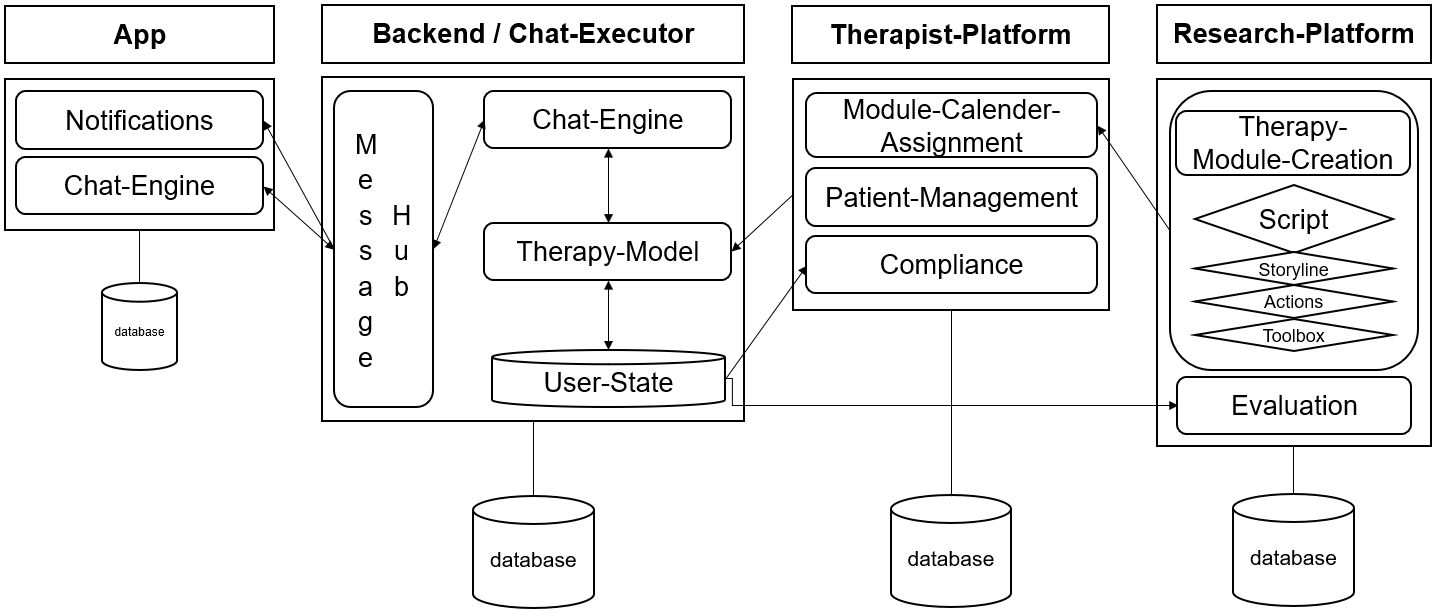
\includegraphics[width=1\textwidth]{pictures/TherapyBuilder}
\caption{Architektur des \emph{TherapyBuilders} (vgl. \citep{benjaminhoff})}
\label{therapyBuilder}
\end{figure}


\subsection{Forscher-Plattform}

Auf dieser Plattform wird die Umsetzung eines studientauglichen digitalen Therapiesystems realisiert. Unter einem studientauglichen digitalen Therapiesystem wird ein System verstanden, welches zur Umsetzung von Therapien eingesetzt werden kann. Die Therapien werden in diesem Fall digital, beispielsweise über ein Smartphone, Tablet oder Computer, bereitgestellt. Die Therapie kann dabei in Form einer Studie evaluiert werden.

Die Forscher-Plattform erlaubt Forschern eine digitale Therapie anzulegen. Diese kann später über die Therapeuten-Plattform der entsprechenden Zielgruppe zugänglich gemacht werden. Eine Therapie setzt sich dabei aus verschiedenen Therapiemodulen zusammen. Ein Therapiemodul ist gleichbedeutend mit der Umsetzung einer Therapiemethode. Der Aufbau des Therapiemoduls lässt sich wie folgt versinnbildlichen.

Das Therapiemodul folgt einer Art Skript (\emph{engl. Script}). In diesem Skript wird festgelegt wann und auf welche Weise ein Dialog zwischen Anwender und Chatbot gestartet wird. Innerhalb des Skripts gibt es verschiedene Handlungsstränge (\emph{engl. Storylines}). Ein Handlungsstrang beschreibt einen Dialog zwischen Nutzer und Chatbot und dessen Verlauf. Der Handlungsstrang kann neben einem normalen Dialog auch aus verschiedenen Aktionen (\emph{engl. Actions}) bestehen, die dem Nutzer bereitgestellt werden um beispielsweise Tagebuch über verschiedene Verhaltensweisen zu führen. Auch kann ein Handlungsstrang Übungen beinhalten, die der Nutzer durchführt. Diese Übungen können dem Nutzer als Werkzeug in einer Art Werkzeugkasten (\emph{engl. Toolbox}) bereitgestellt werden. Somit kann der Nutzer jederzeit auf diese Übungen zugreifen.

Die erstellten Therapiemodule werden an das \emph{Module-Calendar-Assignement} übertragen. Zur Erfassung und Bewertung von Nutzerdaten, werden diese im Backend erfasst und als Nutzerstatus an die Auswertungskomponente \emph{Evaluation} weitergeleitet. Somit kann der Forscher den aktuellen Zustand des Moduls verfolgen. (Vgl. \cite[51\psq]{ben})

Der in dieser Arbeit entwickelte \emph{TMA} wird später in dieser Plattform umgesetzt.  


\subsection{Therapeuten-Plattform}
Die Verwaltung der Patienten findet auf der Therapeuten-Plattform statt. Auf dieser können Patienten hinzugefügt, entfernt sowie verschiedene Therapiemodule ihren Profilen zugeteilt werden. Jedes Probandenprofil enthält eine Darstellung der aktuell zugeteilten und aktiven Therapiemodulen in Form eines Kalenders. Der Therapeut kann anhand dessen nachvollziehen, wie der entsprechende Therapieplan des Patienten aufgebaut ist. Außerdem kann hier auch das Einsehen des Therapiestands des Patienten ermöglicht werden. Die entsprechenden Profildaten werden in einer zugehörigen Datenbank gespeichert. (Vgl. \cite[51\psq]{ben})


\subsection{Backend}
Die Ausführung der Therapiemodule wird durch den \emph{Chat-Executor} gesteuert. Hier werden die Nachrichten der Therapiemodule an die App der entsprechenden Patienten verteilt, sowie die Antworten der Probanden entgegengenommen, gespeichert und verarbeitet. Die erhobenen Daten können in der Therapeuten-Plattform nachvollzogen werden. (Vgl. \cite[51\psq]{ben})

\subsection{App}
Die App wird auf dem Gerät des Patienten installiert. Diese nimmt die Nachrichten entgegen und übersetzt die Darstellung in eine, für Chattechnologien typische, Ansicht. Auch verwaltet sie die Notifications über erhaltene Nachrichten, die den Beginn einer Unterhaltung eines Therapie-Moduls einleiten. Auch leitet die App die Antworten des Nutzers an das Backend weiter.(Vgl. \cite[51\psq]{ben})

\section{Chatbots}

Im Rahmen dieser Arbeit wird unter Chatbots folgende Begriffsdefinition des Oxford Lexikons verstanden.

\quote{A computer program designed to simulate conversation with human users, especially over the Internet.}(Vgl. \cite{chatbotD24:online})

Dies bedeutet, dass ein Chatbot als solchen angesehen wird, sobald Gespräche simuliert werden. Zwischen dem Gesprächspartner und dem Chatbot werden Nachrichten vermittelt die einen Gesprächsverlauf entstehen lassen. Dieser Verlauf kann derart geformt sein, dass dem Nutzer Antwortmöglichkeiten vorgegeben werden und der Chatbot die Möglichkeit hat, entsprechend darauf zu reagieren. Die Eingaben des Nutzers werden im Rahmen dieser Arbeit nicht mit Hilfe von Sprachverarbeitung analysiert und verarbeitet. Viel mehr werden Gesprächsverläufe, ähnlich eines Spielbuchs, vorgegeben und beschrieben. Basierend auf der gewählten Antwort und Entscheidung des Nutzers kann der Gesprächsverlauf beeinflusst werden.